\documentclass[10pt, hyperref={unicode}]{beamer}
\usetheme{CambridgeUS}
\usepackage[utf8]{inputenc}
\usepackage[czech]{babel}
\usepackage[IL2]{fontenc}

\usepackage{times}
\usepackage{listings}
\usepackage{xcolor} 
\usepackage{amsthm, amssymb, amsmath}
\usepackage{multirow}
\usepackage{graphics}
\usepackage[ruled,linesnumbered, noline, longend]{algorithm2e}

\title{Bubble sort}
\author{Dalibor Králik}
\subtitle{Typografie a publikování}
\date{\today}


\begin{document}
    \begin{frame}
        \maketitle
    \end{frame}
    
    \begin{frame}{Obsah}
        
        \tableofcontents
    \end{frame}
    
  
    
    \section{Motivácia}
    \begin{frame}{Motivácia}
         \begin{center}
         Radiace algoritmy sú jednou z najpožadovanejších a najpotrebnejších znalostí každého programátora. Tieto vedomosti sa využívajú na každodennej bázy a je potrebné, aby si tieto znalosti programátor osvojil a využíval ich naplno vo svoj prospech.
         \end{center}
    \end{frame}
    
    \section{Bubble sort - princíp}
    \begin{frame}{Bubble sort - princíp}
    
    
            Viacnásobné prechádzanie pola v jednom smere a výmena susedných prvkov na základe ich veľkostí tzv. prebublávanie
            
          
    
        
    \end{frame}
    
    
    \section{Vizualizácia}
    \begin{frame}{Vizualizícia bubble sortu}
        \begin{figure}
            \centering
             \scalebox{0.07}{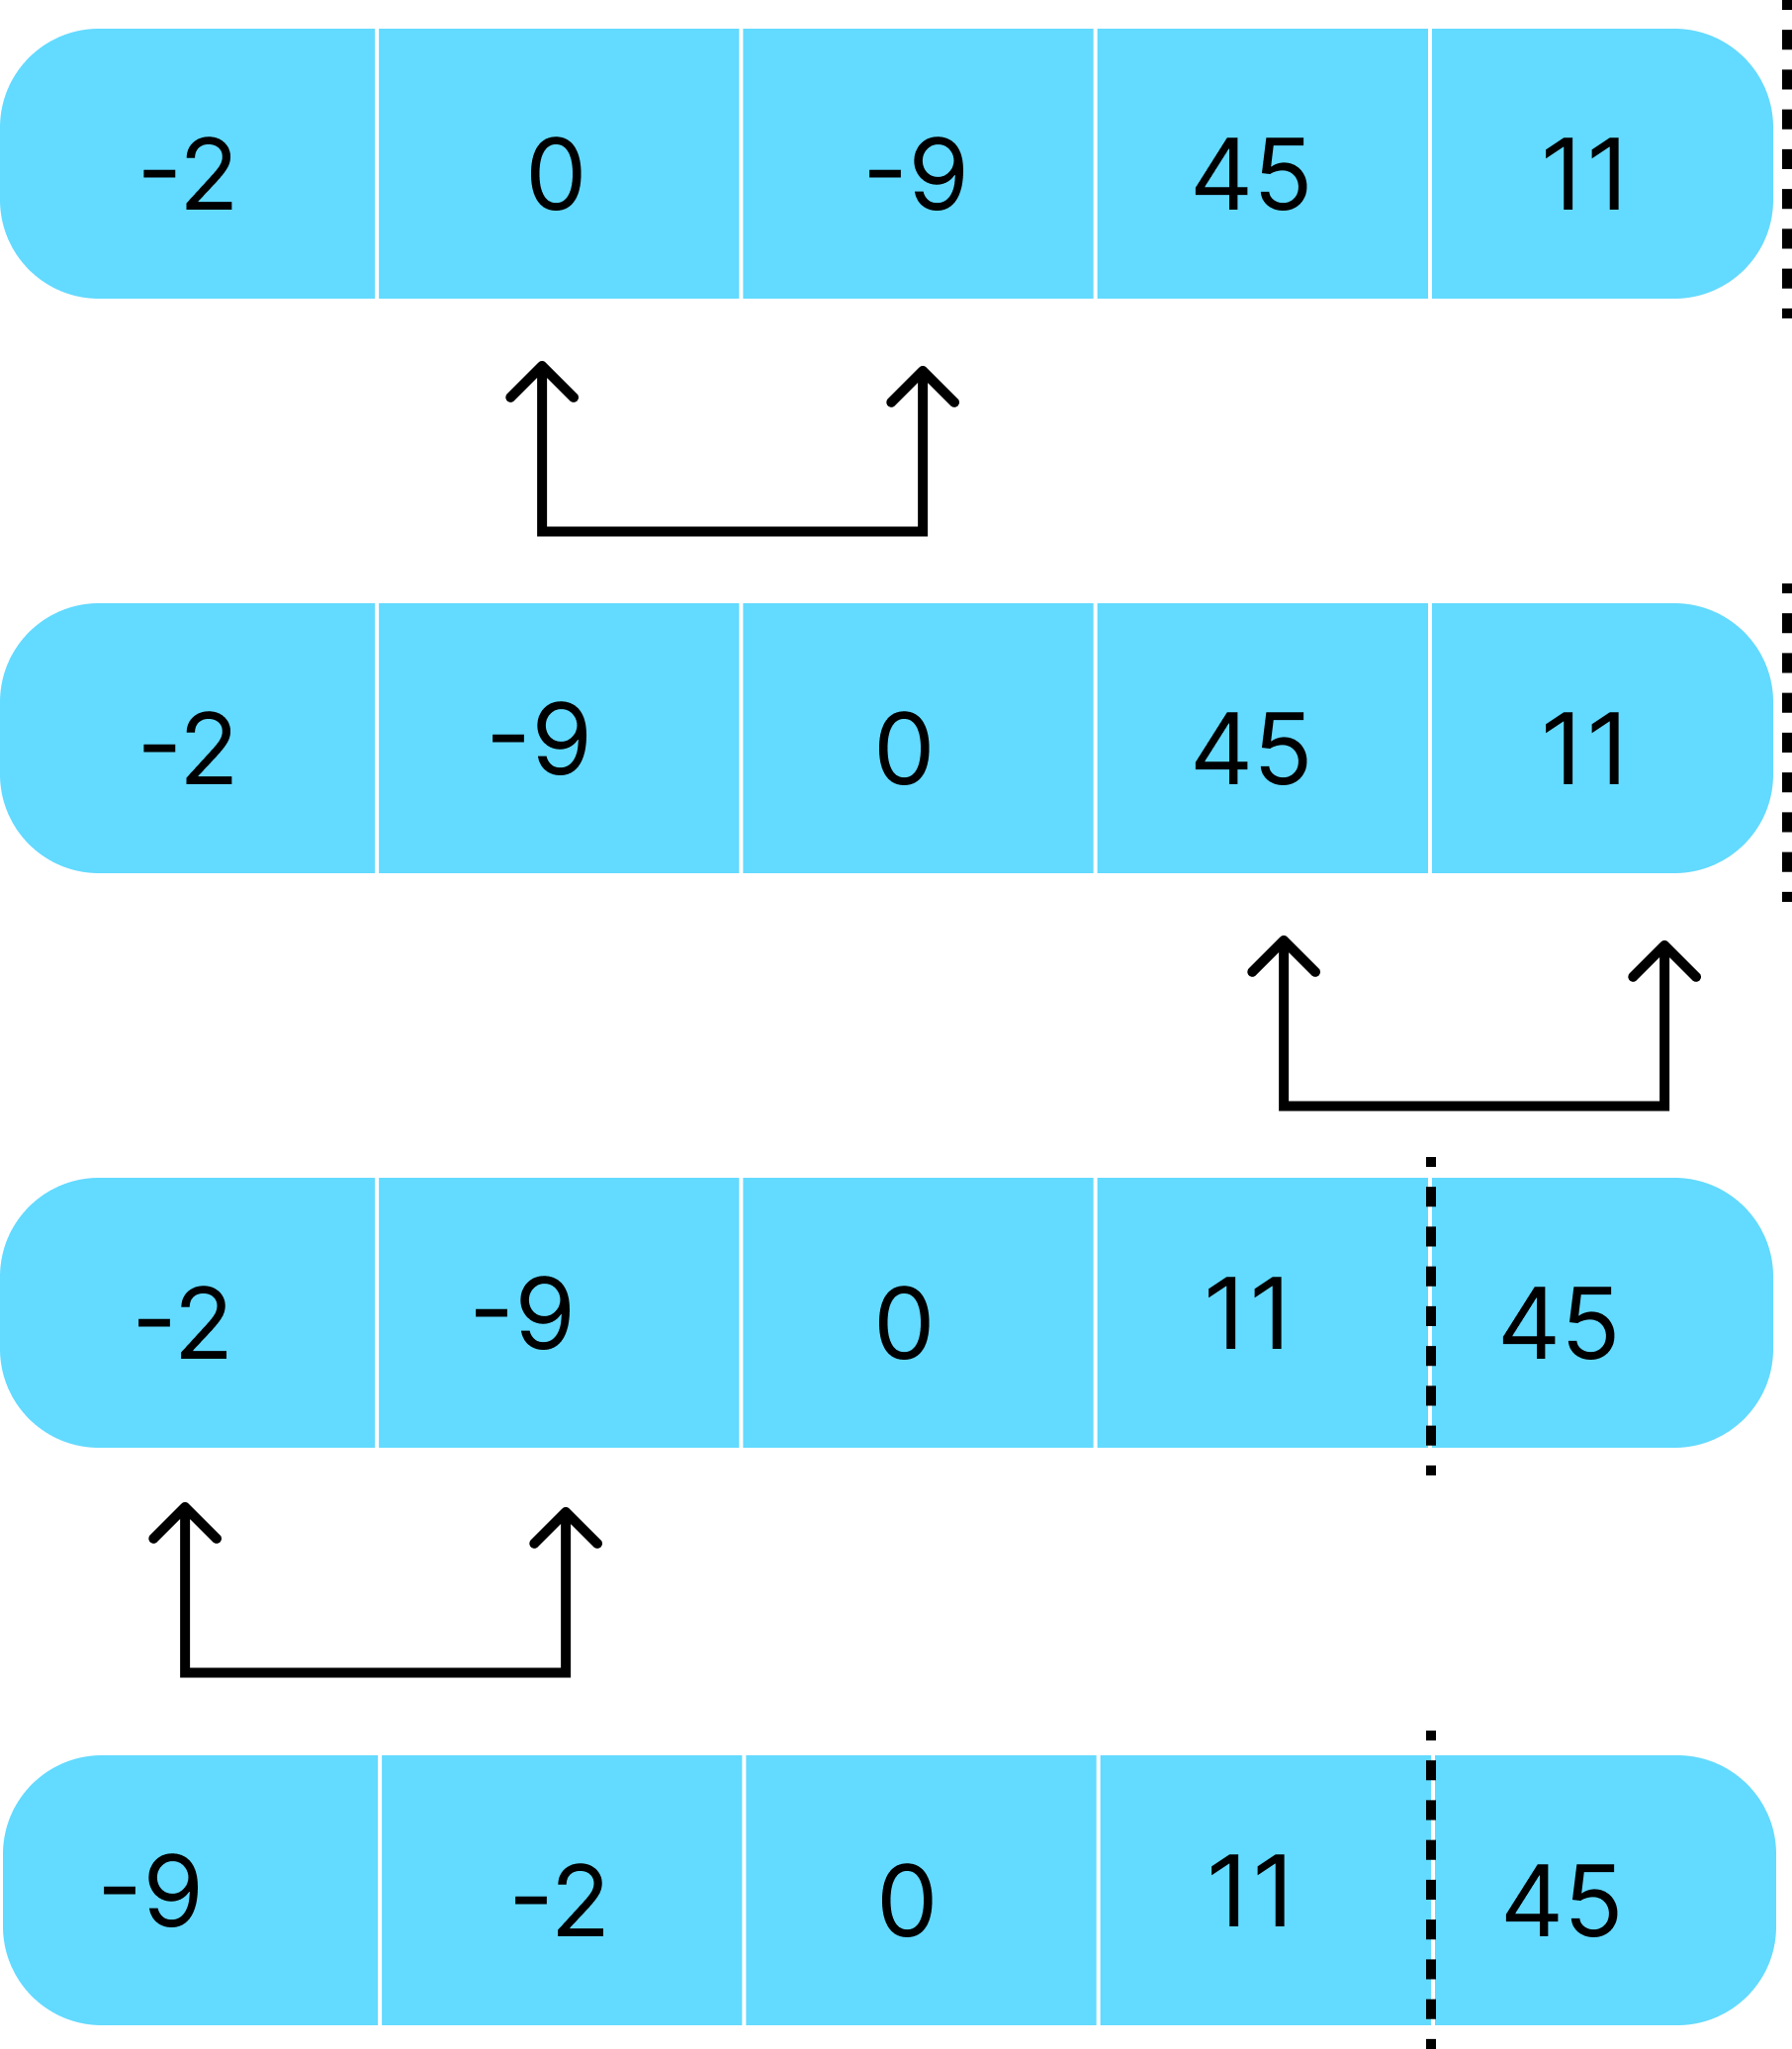
\includegraphics{bubble.png}}
            \caption{Bubble sort}
        \end{figure}
    
        
    \end{frame}
    
    \section{Algoritmus}
    \begin{frame}{Algoritmus}
        \begin{itemize}
            \item Viacnásobné prechádzanie pola v jednom smere a výmena susedných prvkov na základe ich veľkostí tzv. prebublávanie
            
            \item Pri radení vzostupne z ľava, ak je prvom na ľavo väčší ako prvom na pravo tak sa tieto prvky vymenia
            \item Nasleduje porovnávanie ďalšej dvojice
            \item Po ukončení prechodu nasleduje ďalší prechod pola a posunie sa hranica, za ktorou sa nachádza usporiadaná časť pola.
            \item Algoritmus sa ukončí až vtedy, keď sa spraví N-1 prechodov pri N prvkovom poli.
        \end{itemize}
    \end{frame}

    \section{Pseudokód}
    \begin{frame}{Pseudokód python}
        
        \begin{algorithm}[H]
            
            \caption{\textsc{Bubble sort}}
            
            \SetNlSty{}{}{:}
        	\SetNlSkip{-0.6em}
        	
        	
        	\Indp
        	\BlankLine
        	$\textbf{def}\:bubble\_sort(array):$\\
        	\Indp    $index\:=\:len(array)\:-\:1$\\
        	    $\textbf{while}\: index >= 0:$\\
            \Indp    $ \textbf{for}\:j\:in\:range\:(index):$\\
        	\Indp           $\textbf{if}\:array[j]\:>\:array[j+1]:$\\
        	\Indp               $array[j],\:array[j+1]\:=\:array[j+1],\:array[j]$\\
        	\Indm \Indm        $index\:=\: index\: - \: 1$\\
        	\Indm    \Return{$array$}
        	    
    
	
	
        
    
        \end{algorithm}
    \end{frame}


    \section{Časová zložitosť}
    \begin{frame}{Časová zložitosť}
        \begin{itemize}
            \item Časová zložitosť bubble sortu je $O(n^2)$.
            \item Kvadratická zložitosť vzniká vnoreným cyklom v cykle.
        \end{itemize}
    \end{frame}
    
    \section{Použité zdroje}
    \begin{frame}{Použité zdroje}
        \begin{itemize}
            \item Briliant.org - Bubble sort \\
            \href{https://brilliant.org/wiki/bubble-sort/}{\small{\texttt{https://brilliant.org/wiki/bubble-sort/}}}
            
        \end{itemize}
    \end{frame}

\end{document}
